\documentclass{report}

%----- Packages to be imported
\usepackage{physics}
\usepackage{amsmath}
\usepackage{amssymb}
\usepackage{epsfig}
\usepackage{setspace}
\usepackage{fancyhdr}
\usepackage{graphicx}
\usepackage{color}
\usepackage{chemformula}
\usepackage{tablefootnote}
\usepackage{threeparttable}
\usepackage{subfigure}
\usepackage{float}
\usepackage[toc,page]{appendix}
\usepackage[left=2.5cm,top=3cm,right=2.5cm,bottom=3cm,bindingoffset=0.5cm]{geometry}

\pagestyle{plain}

\begin{document}

\setcounter{secnumdepth}{4}
	%\sets numbering upto 4th level in chapter,section, subsection, subsubsection
\setcounter{tocdepth}{4}
	%\makes levels upto the 4th appear in the table of contents

%---- Roman page numbering for frontmatter
	\pagenumbering{roman}
	\setcounter{page}{1}
\thispagestyle{empty}
\begin{titlepage}

	\begin{center}

	\singlespacing
	\textbf{TITLE}\\
	\doublespacing
	
	by\\
	
	\textbf{Kraig Andrews}\\
	Ph.D. Disseration Prospectus\\ 

	\end{center}

\end{titlepage}
	\begin{center}
\textbf{ABSTRACT}
	
	
	\singlespacing
\textbf{Quantum Transport Properties and Scattering Mechanisms in Transition Metal Dichalcogenides}\\
	\doublespacing
	
	by\\
	
	\textbf{Kraig J. Andrews}\\
	February 2016\\
\end{center}
\begin{tabular}{ll}	
Advisor: & Dr. Zhixain Zhou\\
Major:   &Physics\\
Degree:  &Doctor of Philosophy
\end{tabular}
\bigskip

\noindent Two-dimensional materials have garnered much interest since the isolation of graphene. Since then layered materials, such as transition metal dichalcogenides (TMDs) have been studied extensively. However, several key problems have yet to be solved. In this study we propose using methods developed to decrease and minimize contact resistance through a novel approach of 2D/2D contacts and \hbn encapsulation to study how the mobility and intrinsic properties are affect by $p$-doping \ch{WSe2} device channels. Preliminary results show contact resistance as low as $0.185\unita{k\Omega\cdot\mu m}$ using degenerately doped contacts and field-effect mobilities of $\sim 200\cmvs$ and $\sim 650\cmvs$ at $T=300\unita{K}$ and $T=5{K}$, respectively using this 2D/2D contact \hbn encapsulation method. In addition, this method is intended to improve mobility at both room temperature for device applications and at low temperatures ($\sim 4\unita{K}$) to study the integer quantum hall effect (IQHE) and the corresponding related quantum oscillations (Shubnikov-de Haas oscillations) to determine information related to quantum scattering times, effective cyclotron mass, and the geometry of the Fermi surface. 

	\newpage
\begin{center}
{\bf ACKNOWLEDGEMENTS}
\end{center}

Acknowledgements here...

	\renewcommand{\contentsname}{Table of Contents}
        \tableofcontents
	\newpage
        \addcontentsline{toc}{section}{List of Figures}
	\listoffigures 
	\newpage
	\addcontentsline{toc}{section}{List of Tables}
	\listoftables
	\newpage
	\pagenumbering{arabic}
         \pagestyle{fancy}
        \fancyhead{} 
	\fancyfoot{} % clear all header and footer fields
        \chead[]{\thepage}
        \renewcommand{\headrulewidth}{0pt}
         \renewcommand{\footrulewidth}{0pt}
	%\pagestyle{myheadings}%supposed to put pg number in header
	%\pagenumbering{arabic}
	\fancypagestyle{plain}{%
	\fancyhf{} % clear all header and footer fields
	\fancyhead[C]{\thepage} % except the center
	\renewcommand{\headrulewidth}{0pt}
	\renewcommand{\footrulewidth}{0pt}}

%---- End of front matter
	\pagenumbering{arabic}
	\chapter{Introduction}\label{sec:intro}
\section{Early Semiconductors}\label{sec:early_semicond}
The development of microelectronics revolutionized the world in the latter half of the twentieth century. The term semiconductor, in the sense it is known today, first appears in literature in 1911 \cite{Koenigsberger_AnnalenDerPhysik1911}. Initially, work on the subject was rather pessimistic. However, in the years following Word War II breakthroughs began shed light on the possible applications and the underlying physics involved, such as the ideas of \emph{instrinsic} and \emph{extrinsic} semiconductors \cite{Busch_EuroJournPhys1989,Lark_AAAS1954,Wilson_Royal1931a,Wilson_Royal1931b}. \\

%\noindent
The history of semiconductors and transistors is a well documented subject. The first transistor was constructed at Bell Labs in 1947 using polycrystalline germanium. Shortly thereafter one was developed using silicon. Throughout the following years, these devices were improved on by replacing polycrystalline with single crystals \cite{Neamen_Semiconductor_Physics2003}. Then Jack Kilby demonstrated the first  \ac{IC} in 1958, for which he would win the Nobel Prize in physics \cite{Lukasiak_JorunTelcomm2010, Kilby_Patent1959}. The scale of \acp{IC} grew rapidly in the subsequent years. Initially only a few transistors could fit on a chip (small-scale integration), in stark contrast to modern-day chips that contains billions of transistors \cite{Moore_Electronics1965, Clarke_EEtimes2005}. Growth continued at a rapid pace, but eventually it was realized that some limits, material and integration based, existed in silicon and other commonly used materials \cite{Meindl_Science2001, Schulz_Nature1999}. In part, these limitations increased the interest in alternative materials. As a result widespread and renewed interest has led to a breadth information and results on a wide range of materials and their applications.

\section{Graphene as a New \Td Material}\label{sec:graphene}
Layered materials have existed for a long time, and have been studied over the last few centuries \cite{Golden_EarthSci2013,Brodie_Royal1859}. In recent decades the scientific study of graphite (3D) has led to new forms of materials, such as carbon nanotubes (1D) and fullerenes (0D) \cite{Kroto_Nature1985, Balleste_Nanoscale2011,Iijima_Nature1991}. However, only more recently have scientists began to understand the potential of such layered materials and their potential technological applications. After attempting unsuccessfully to synthesize few-layer graphite during the 1960s, only around 10-50 layers were able to be synthesized, a breakthrough was finally acheived \cite{Balleste_Nanoscale2011}. This most notably began with the synthesis of monolayer graphene \cite{Novoselov_Science2004}.

\subsection{Properties of Graphene}\label{subsec:graphene_properties}
To date, graphene's properties have been the focus of much research, both theoretical and experimental. It has been one of the primary driving forces in study of `relativistic' condensed matter physics due to its low dimensionality and its band structure that allows electrons to mimic relativistic particles confirming the appearance of several relativistic phonomena \cite{Geim_NatureMat2007,Geim_Nature2005,Zhang_NatPhys2011,Williams_Science2007}. In its most basic sense, graphene is composed of a single layer of carbon atoms arranged in \td honeycomb lattice (see fig.~\subref*{fig:graphene_honeycomb}) It has a Young's modulus of $~100\unita{GPa}$ (several times more than steel) with a breaking force that is $13\%$ of its Young's modulus \cite{Bertolazzi_ACSnano2011, Akinwande_NatureComm2014}. Its stength is due, in part, to its strong in-plane carbon (\ch{C}) bonds. In addition, graphene can sustain elastic deformations of 20\% due to its \td nature and it has high pliability \cite{Balleste_Nanoscale2011}. These mechanical properties are of interest because graphene lies in the extreme ranges of many metrics considering its size and dimensionality.\\

%\noindent 
Aside from its mechanical properties, graphene's transport properties were another reason why the material was so appealing. Graphene's mobility is several times that of silicon's (electron mobility $\mu\sim 1400\cmvs$, hole mobility $\mu\sim 450\cmvs$ at room temperature). Experimental results have shown graphene mobility around $15,000\cmvs$ with a potential theoretical limit of $200,000\cmvs$ \cite{Dargys_Encylco1994,Akinwande_NatureComm2014,Si_Properties}. The upper theoretical limit imposed on mobility is due to scattering, however, these high mobilities are achieved mainly because electrons in graphene act very much like photons in their mobility due to their lack of mass. This enables them to travel sub-micron distances without scattering \cite{Novoselov_NatureMat2007}. In reality, there are other limiting factors that need to be considered such as the quality of graphene and scattering with the substrate, for example. 
\begin{figure}[ht]
	\centering
	\subfloat[]{
		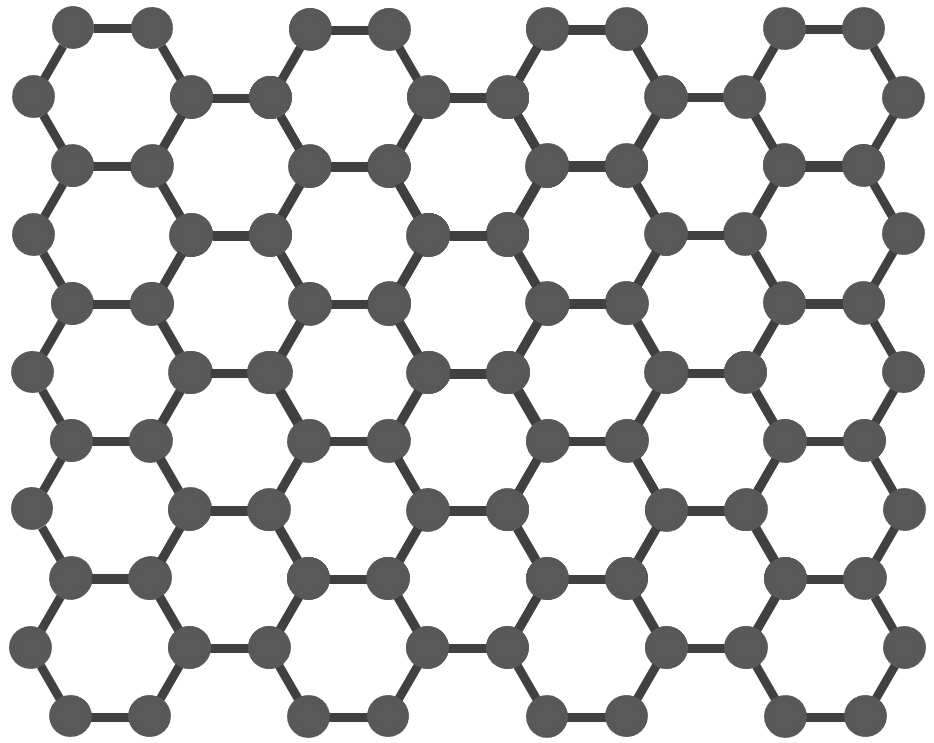
\includegraphics[height=4cm,width=5cm]{figs/intro/graphene_honeycomb}
		\label{fig:graphene_honeycomb}
	}
	\qquad
	\subfloat[]{
		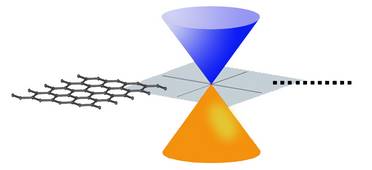
\includegraphics[height=4cm,width=6cm]{figs/intro/graphene_bandgap}
		\label{fig:graphene_bandgap}
	}
	\caption[Lattice and band structure of graphene]{\protect\subref{fig:graphene_honeycomb} Graphene: a layer of carbon atoms in a honeycomb lattice. \protect\subref{fig:graphene_bandgap} One of the most unusual features of graphene is that its conduction and valence bands meet at a point, meaning that in single-layer graphene there is no bandgap (Figures obtained from \cite{Berkley_Online2009}).}
	\label{fig:graphene_structures}
\end{figure}

\subsection{Band Structure of Graphene}\label{subsec:graphene_bandstructure}
%\noindent 
Despite its impressive properties, the main drawback of graphene is its lack of bandgap. As this became known, the prospect of using graphene for the fabrication to \acp{IC} became unlikely. In graphene the conduction and valence bands touch at a single point as shown in fig.~\subref*{fig:graphene_bandgap} \cite{Wallace_PhysRev1947}. Ultimately, the lack of a bandgap means that the current on/off ratio is low and is unappealing for logical circuit applications \cite{Xu_ChemRev2013}. However, graphene exhibits some interesting properties as a result of having no bandgap, particularly as it pertains to its optical properties. The material's band structure allows for absorption of light over a large range of the electromagnetic spectrum, ranging from infrared ($<1.65\unita{eV}$) to ultraviolet ($>3.2\unita{eV}$), offering potential electronic-photonic device applications \cite{Xia_NatureNano2009,Wang_Science2008,Geim_NatureComm2011}. Since a direct use in logical circuits is not practical researchers have moved on to look for `\td materials beyond graphene.' Several attempts at some derivatives of graphene-like materials have been studied, but for the most part they do not seem promising for use in logical circuits \cite{Takeda_PhysRev1994,Cahangirov_PhysRevLett2009}. As of late, research has been concentrated on \td materials, namely transition methal dichalcogenides, as a candidate in \acp{IC} and other potential device applications.

\section{\Td Materials: Transition Metal Dichalcogenides}\label{sec:tmds}
Commonly referred to \td materials beyond graphene, transition metal dichalcogenides (TMDs) have garnered much interest in recent years. \acp{TMD} were studied previously, however, they have gained renewed interest due to their properties \cite{Frindt_Royal1963,Fivaz_PhysRev1967,Mattheiss_PhysRevB1973,Wilson_AdvPhys1969}. \acp{TMD} consist of hexagonal layers of metal (\ch{M}) atoms in between two layers of chalcogen (\ch{X}) atoms (see fig.~\subref*{fig:tmd_hexagonal}), such that the stoichiometry of the material is \ch{MX2} \cite{Xu_ChemRev2013}. The material is dependent on the type of transition metal, typically one of: \ac{Mo}, \ac{W}, \ac{Nb}, \ac{Re}, \ac{Ni}, or \ac{V}, and two chalcogen atoms, typically one of: \ac{S}, \ac{Se}, or \ac{Te} \cite{Wilson_AdvPhys1969,Wells_Oxford1984}. The most commonly studied variations of \acp{TMD} are \ac{MoS2}, \ac{WSe2}, and \ac{WS2}. These materials are commonly stacked together involving van der Waals interactions between adjacent sheets and covalent bonding within each individual sheet (see fig.~\subref*{fig:tmd_layer}) \cite{Xu_ChemRev2013}.
\begin{figure}[ht]
	\centering
	\subfloat[]{
		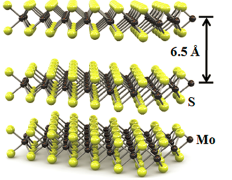
\includegraphics[height=4cm,width=6cm]{figs/intro/tmdlayered}
		\label{fig:tmd_layer}
	}
	\qquad
	\subfloat[]{
		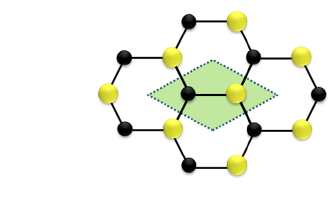
\includegraphics[height=4cm,width=6cm]{figs/intro/tmdhexagonal}
		\label{fig:tmd_hexagonal}
	}
	\caption[Hexagonal lattice structure of \acs{TMD}]{\protect\subref{fig:tmd_layer} The atomic structure of a layered \acs{TMD}, depicting \acs{MoS2}. Each sheet is composed of three atoms with \ch{Mo} sandwiched in between two \acs{S} atoms, \acs{S}-\acs{Mo}-\acs{S}. \protect\subref{fig:tmd_hexagonal} Top view of a \acs{TMD} (\acs{MoS2}) lattice. (Figures obtained from \cite{Kis_NatureNano2011})}
\end{figure}
%\noindent 
\acp{TMD} have been found to exhibit a wide variety of interesting properties, including either being a metal or insulator, and displaying the topological insulator effect, superconductivity, and thermoelectricity \cite{Lang_ACSnano2012,Zhang_AdvMat2012,Xie_AppPhysLett2009,Gamble_JournChemPhys1975}.

\subsection{Band Structures of \acp{TMD}}\label{subsec:tmd_properties}
%\noindent
\noindent As stated in sec.~\ref{subsec:graphene_bandstructure}, one important propert as it pertains to applications for logical circuits is the material's band structure. One of the main reasons \acp{TMD} have been so extensively studied lately is due to the fact that, unlike graphene, they do exhibit a bandgap. The bandgaps in some commonly used \acp{TMD} is interesting because of the transition from an indirect to a direct bandgap as the layered thickness decreases. Fig.~\ref{fig:mos2_bandstructure} illustrates this, for bulk and few-layer \acs{MoS2} there is an indirect band gap while for monolayer \acs{MoS2} there is a direct bandgap. This unusual structure results in some unique optical properties making monolayer \acs{TMD} promising candidates for optoelectronic devices \cite{Cheng_NanoLett2014,Conley_NanoLett2013}. Table~\ref{table:band_gaps} summarizes some \acs{TMD} bandgap energies that are of considerable interest to the device fabrication process. 
\begin{figure}[ht]
	\centering
	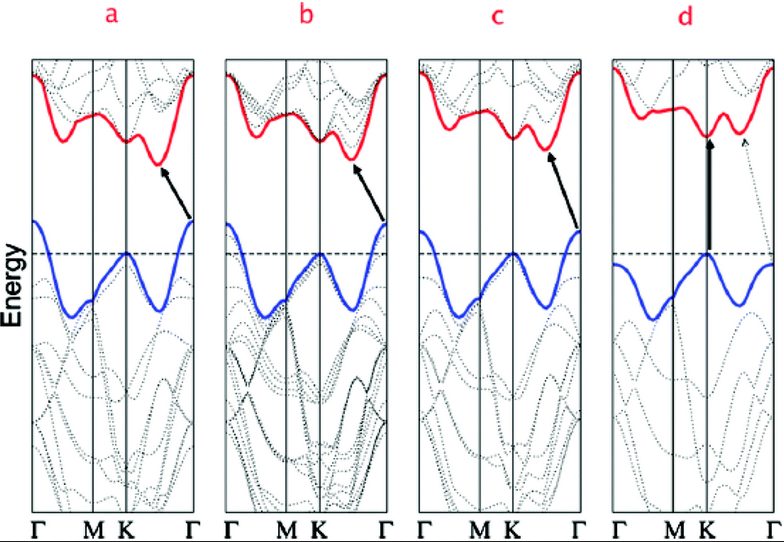
\includegraphics[height=5cm,width=8cm]{figs/intro/mos2_bandstructure}
	\caption[Band structures of \acs{MoS2}]{Calculated band structures of (a) bulk \acs{MoS2}, (b) four-layer \acs{MoS2}, (c) bilayer \acs{MoS2}, and (d) monolayer \acs{MoS2}. Here the solid arrows indicate the lowest energy transitions. (Taken from \cite{Lee_Nanoscale2014}, originally appeared in \cite{Splendiani_Nanolett2010})}
	\label{fig:mos2_bandstructure}
\end{figure}
 
 \begin{table}[ht]
	\centering
	\begin{threeparttable}
	\begin{tabular}{c c c}
		%\hline\hline
		\toprule
		2D material & theoretical $E_g\,(\mathrm{eV})$ & experimental $E_g\,(\mathrm{eV})$ \\ [0.5ex]
		%\hline
		\midrule
		graphene & 0 & 0 \\
		bilayer graphene & 0 & 0\\
		bulk $h$-\ch{BN} & - & 5.97 \cite{Kubota_Science2007}\\
		monolayer $h$-\ch{BN} & - & 6.07 \cite{Kim_NanoLett2011}\\
		few layer (2-5) $h$-\ch{BN} & - & 5.92 \cite{Song_NanoLett2010}\\
		bulk \acs{MoS2} & 1.2\tnote{a,b}\,\,\,\,\, \cite{Mak_PhysRevLett2010,Gourmelon_Solar1997} & 1.0-1.29\tnote{b}\,\,\, \cite{Mak_PhysRevLett2010,Gourmelon_Solar1997}\\
		monolayer \acs{MoS2} & $\sim 1.90$\tnote{a,c}\,\,\,\,\, \cite{Fortin_JournChemSolids1982} & $\sim 1.90$\tnote{b}\,\,\, \cite{Fortin_JournChemSolids1982}\\
		bulk \acs{WS2} & $\sim 1.30$\tnote{a,b}\,\,\,\,\, \cite{Mak_PhysRevLett2010,Kuc_PhysRevB2011} & $\sim 1.35$\tnote{c}\,\,\, \cite{Mak_PhysRevLett2010,Kuc_PhysRevB2011}\\
		monolayer \acs{WS2} & $\sim 2.10$\tnote{a,c}\,\,\,\,\, \cite{Ma_JournChemPhys2011} &-  \\
		bulk \ch{WSe2} & - & $\sim1.20$\tnote{b}\,\,\,\,\, \cite{Wang_NatureNano2012}\\
		monolayer \ch{WSe2} &- & $\sim1.7$\tnote{c}\,\,\,\,\, \cite{Wang_NatureNano2012}\\ [1ex]
		%\hline
		\bottomrule
	\end{tabular}
	\begin{tablenotes}
		\item[a] Theoretical calculations based on first-principles calculations using \ac{DFT}.
		\item[b] Indirect bandgap semiconductor.
		\item[c] Direct bandgap semiconductor.
	\end{tablenotes}
	\caption[Band gaps of typical \acp{TMD} and other materials]{Summary of the bandgaps of typical monolayer, bilayer, and bulk \acp{TMD} and $h$-\ch{BN} materials. Table adapted from ref.~\cite{Xu_ChemRev2013}.}
	\label{table:band_gaps}
	\end{threeparttable}
\end{table}

\section{Current Challenges in \acp{TMD} and Beyond}\label{sec:tmds_and_beyond}
There are several challenges facing the advancement of study of \acp{TMD}. One of these is the development of low contact resistance devices. The formation of a \ac{SB} occurs when making electrical contacts \cite{Fang_NanoLett2012,Das_AppPhysLett2013}. This problem affects many aspects of the growth of \acp{TMD}, low contact resistance devices are essential for the study of intrinsic transport properties and performance limits of devices. Two main approaches exist for achieving low-resistance metal-semiconductor contacts. The first of these is lowering the \ac{SBH} by choosing metals with proper work functions. Finding metals with the proper work function to minimize the \acs{SBH} while still maintaining a high conductivity has proven to be difficult \cite{Liu_ACSnano2012,Das_NanoLett2012}. If a proper work function metal were to be found that met the requirements for current \acs{TMD} performance the effect of lowering the \acs{SBH} may still be diminished due to Fermi level pinning \cite{Gong_NanoLett2014}. Therefore, another method to achieve low-resistance contacts is desirable. The second approach used to achieve low-resistance contacts is to degenerately dope the contact regions. Heavily doping the contact region effectively decreases the \acs{SB} width \cite{Suh_NanoLett2014}. However, this too, has its own challenges associated with it. One possible way to overcome the problems and tune the \acs{SB} is to use a buffer layer and covering with a material such as \hbn or graphene \cite{Geim_Nature2013,Farmanbar_PhysRevB2015,Kappera_NatureMat2014,Farmanbar_arxiv2016}. This second approach has shown promise in reducing the contact resistance and lowering the \acs{SB} while still maintaining high carrier mobility (see ch.~\ref{chap:results}). \\ \\

%\noindent
Aside from the commonly used \td materials like \ch{MoS2} and \ch{WSe2}, \ac{BP} has begun to show promise. Bulk \acs{BP} has a direct bandgap of $\sim 0.3\unita{eV}$, which is expected to increase to $\sim 2.0\unita{eV}$ as the thickness approaches monolayer \cite{Keyes_PhysRev1953,Maruyama_PhysB1981,Tran_PhysRevB2014}. In the past few years, few-layer black phosphorus has been shown to have desireable room temperature field-effect mobility ($\sim 1,000\cmvs$ for $\sim 10$ layer \acs{BP} and $\sim 200\cmvs$ for $5\unita{nm}$ \acs{BP}) \cite{Li_NatureNano2014,Koenig_AppPhysLett2014,Xia_NatureComm2014}. \acs{BP} has shown potential for applications to thin-film electronics and infrared optoelectronics due to its bandgap energy range \cite{Li_NatureNano2015,Xia_NatureComm2014}. In addition, the high mobility measurements have recently allowed for measurements of novel quantum physics, opening the door to further study of intrinsic channel properties of \acp{TMD}.


%\section{Hall Effect}\label{sec:hall_effect}
%Give a brief overview of the history
%\subsection{Overview}\label{subsec:hall_overview}
%\subsection{Theoretical Background}\label{subsec:hall_theory}
%Some useful references for this section \cite{Hall_AmerJournMath1879,Schroder_Semiconductor2006,Kittel_IntroSolidState2005,Ashcroft_SolidStatePhysics1978,Melissinos_Experiments1966,Baumgartner_HallEffect2006} %introduction and preliminary information
	\chapter{Experimental Details}\label{chap:exp_details}

\section{Nano-device Fabrication}\label{sec:device_fab}
\subsection{Subsect 1}\label{subsec:subsec1}
 %chap2
	\chapter{Results and Discussion of Experiment}\label{chap:chap3}
\section{Section Heading}\label{sec:heading2} %chap3
	\chapter{Future Works and Conclusion}\label{chap:conclusion}
\section{Heading}\label{sec:heading31}

\section{Limitations}\label{sec:limitations} %conclusions

%---- References and bib data
	\bibliographystyle{plain}
	\bibliography{refs/database}

	\begin{appendices}
		\appendix
		\appendix
Text goes here...
	\end{appendices}

\end{document}
